\chapter{ローカルデータベースにおける検索機能とその処理時間}

モジュール組み立てにおいて、読み出し試験は複数回行われ、一回の試験で行う項目も複数存在する。
そのため、生産時には試験結果が数多くデータベースにアップロードされることになる。
4章で述べたように、任意のタイミングで必要な結果を取得できる検索機能を実装した。詳細について以下に示す。

\section{実装方法}
今回の実装では、一般的にウェブで用いられているフリーワードの検索エンジンのような機能を実装しようと考えた。
ユーザの操作を最小限にし、直感的かつ柔軟な検索ができるようにするためである。

読み出し試験において、対象とする検索キーワードを以下の項目に絞った。
システムにおいて、アップロードされた試験結果に関わるデータベース内の情報は後から編集する機能はサポートしない方針を取っている。
品質試験の結果が後から上書きされては、結果の信頼性を失うと考えているからである。
そのため、ユーザが対象としたい検索キーワードは以下の項目に限られ、検索キーワードとしてサポートすれば十分であると考えた。

\begin{itemize}
  \item モジュール及びFEチップのID.
  \item 読み出し試験項目(例:\texttt{std$\_$digitalscan})
  \item 読み出し試験者.
  \item 読み出し試験場所.
  \item 試験日時.
  \item タグ機能を用いてつけられたタグ.
\end{itemize}

そこで実装方法として、以下の2つを考えた。

\begin{enumerate}
  \item 各試験に関する情報をプログラム上で配列に保持し、検索キーワードが含まれるかを確認する方法.
  \item 各試験に関する情報を持つドキュメント、コレクションを予め作成、それを参照し検索を行う方法.
\end{enumerate}

これらについて以下で詳細を説明する。

\subsection{方法1: Pythonリストを用いた一致確認}
Pythonリストを使う実装の場合、以下のような流れで検索処理を行う。
\begin{enumerate}
  \item ユーザが検索キーワードを入力し、処理を実行.
  \item アップロードされた全ての読み出し試験結果に関する情報を取得.
  \item 各試験結果に関連する情報をPythonリストに保持、検索キーワードとの一致を確認、試験を選別.
  \item ブラウザーに送信.
\end{enumerate}

アルゴリズムのイメージを図\ref{search_python_list}に示す。
この方法では、データベース内の試験結果とアプリケーションの関数内だけで全ての処理を行うことが可能なため、シンプルな実装方法であると言え、直感的に始めに思いつく方法であった。

\begin{figure}[bpt]
  \begin{center}
    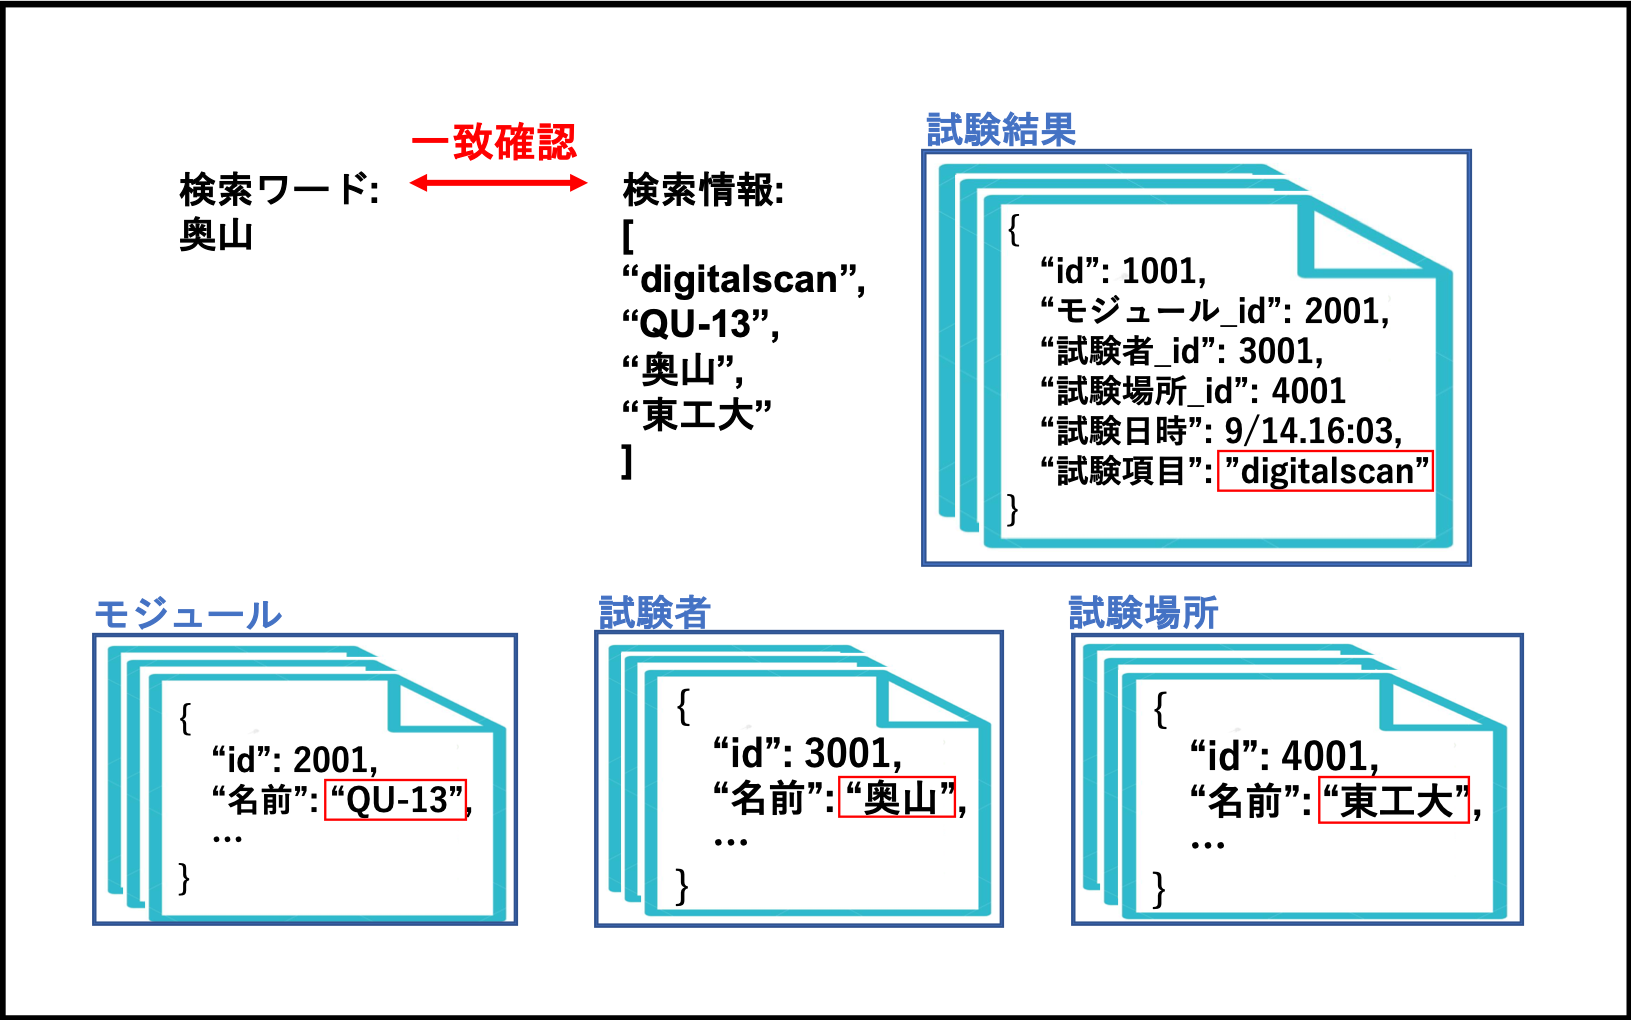
\includegraphics[width=12cm]{search_python_list}
    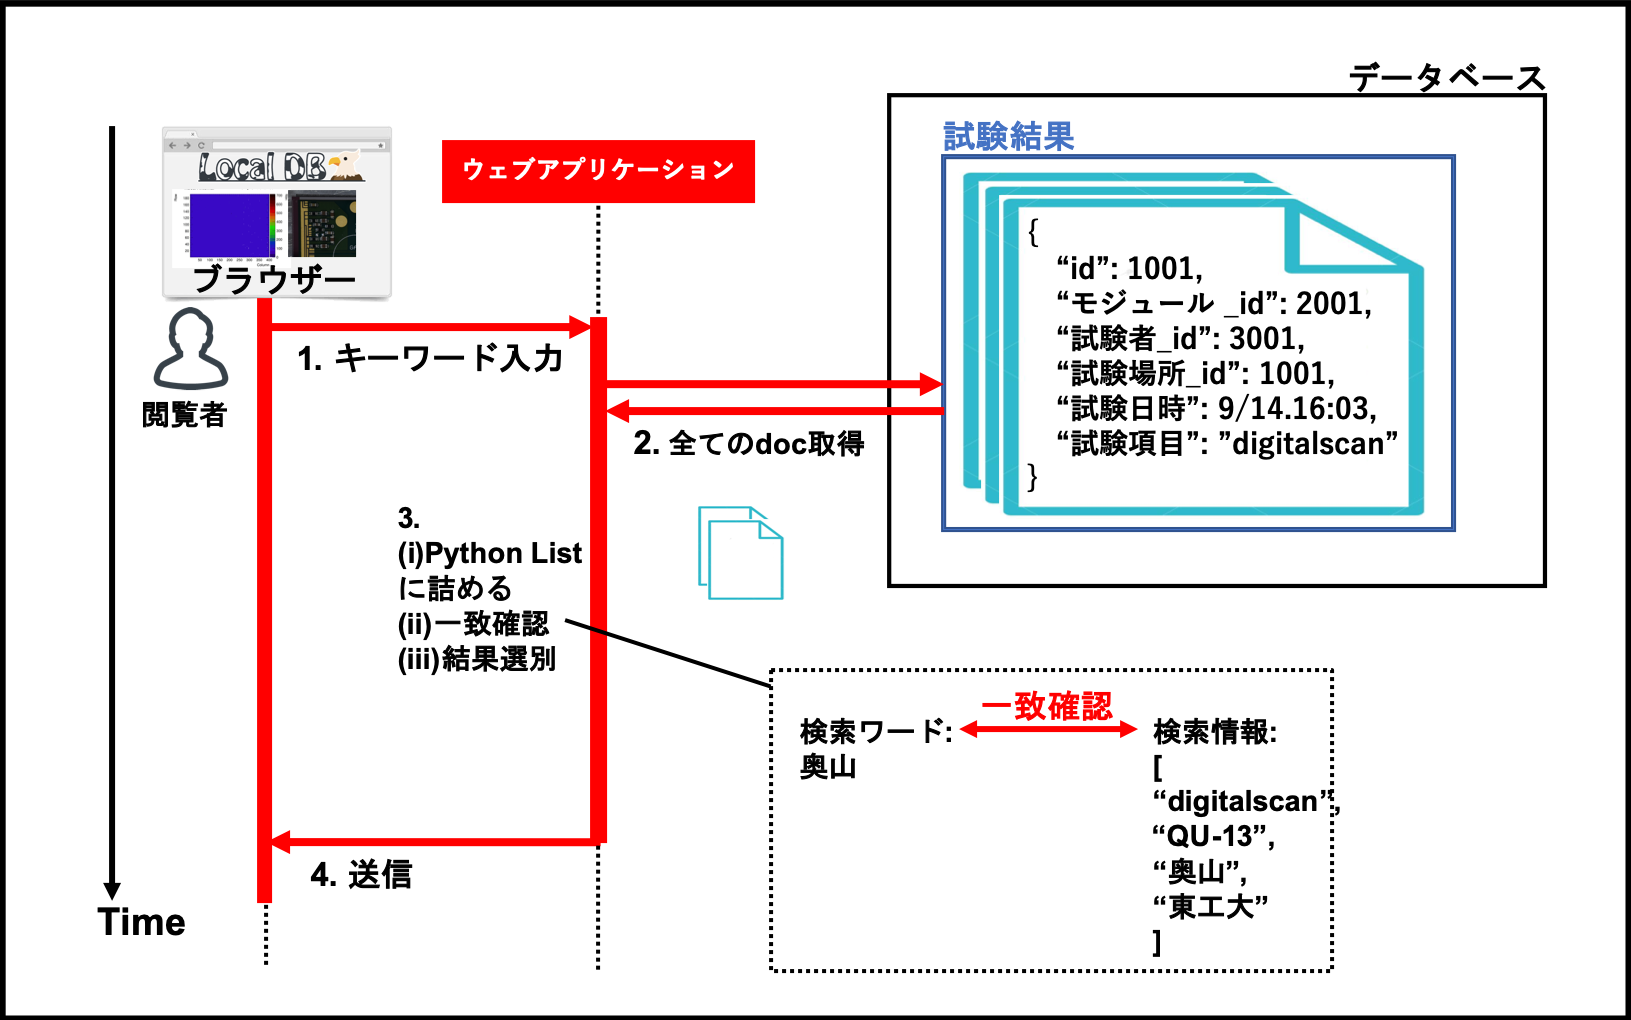
\includegraphics[width=12cm]{search_python_list_flow}
  \caption[検索機能実装方法1:Pythonリストを用いた場合]
{検索機能実装方法1:Pythonリストを用いた場合の検索処理のイメージ図。上図は各コレクションと保存されている情報の例を示しており、下図は実際に検索を行った時の処理の流れを表している。上図中の赤枠で囲われた情報のように検索対象となる名前の情報は複数のコレクションにまたがって保存されている。各試験結果に対してこれらの情報を集めリスト内に保持し、各要素とキーワードとの一致を確認することで検索処理を行う。}
  \label{search_python_list}
  \end{center}
\end{figure}

しかしこの方法を試験実装したところ、ドキュメント数の増加に対して検索処理時間を大きく要してしまう問題が発生した。
図\ref{search_python_list_problem}のようにデータベース内の構造は複数のコレクションを跨いで情報を保持しているため、試験結果全てに対してリアルタイムでこの処理を行うと、検索時間が大きくかかってしまう。
このシステムのデータ構造においては、表\ref{localdb_structure}において各試験結果の情報を保存するtestRun、componentとtestRunの関係を保存するcomponentTestRunの構造による遅延であると考えられる。
試験結果数を$n$とすると、testRunが$n$、componentTestRunがぞれぞれ$O(n)$のドキュメント数を持つことになる。
これらのドキュメントを全て検索し、一致確認を行うと全体で$O(n^2)$の時間がかかる。イメージを図\ref{search_python_testRun}に示す。
この実装方法について、ドキュメント数と処理時間の関係を測定したところ、図\ref{searching_time_python_list}のようになり、確かにドキュメント数に対して2次的に増加していることが分かる。測定の詳細については後述する。
\begin{figure}[bpt]
  \begin{center}
    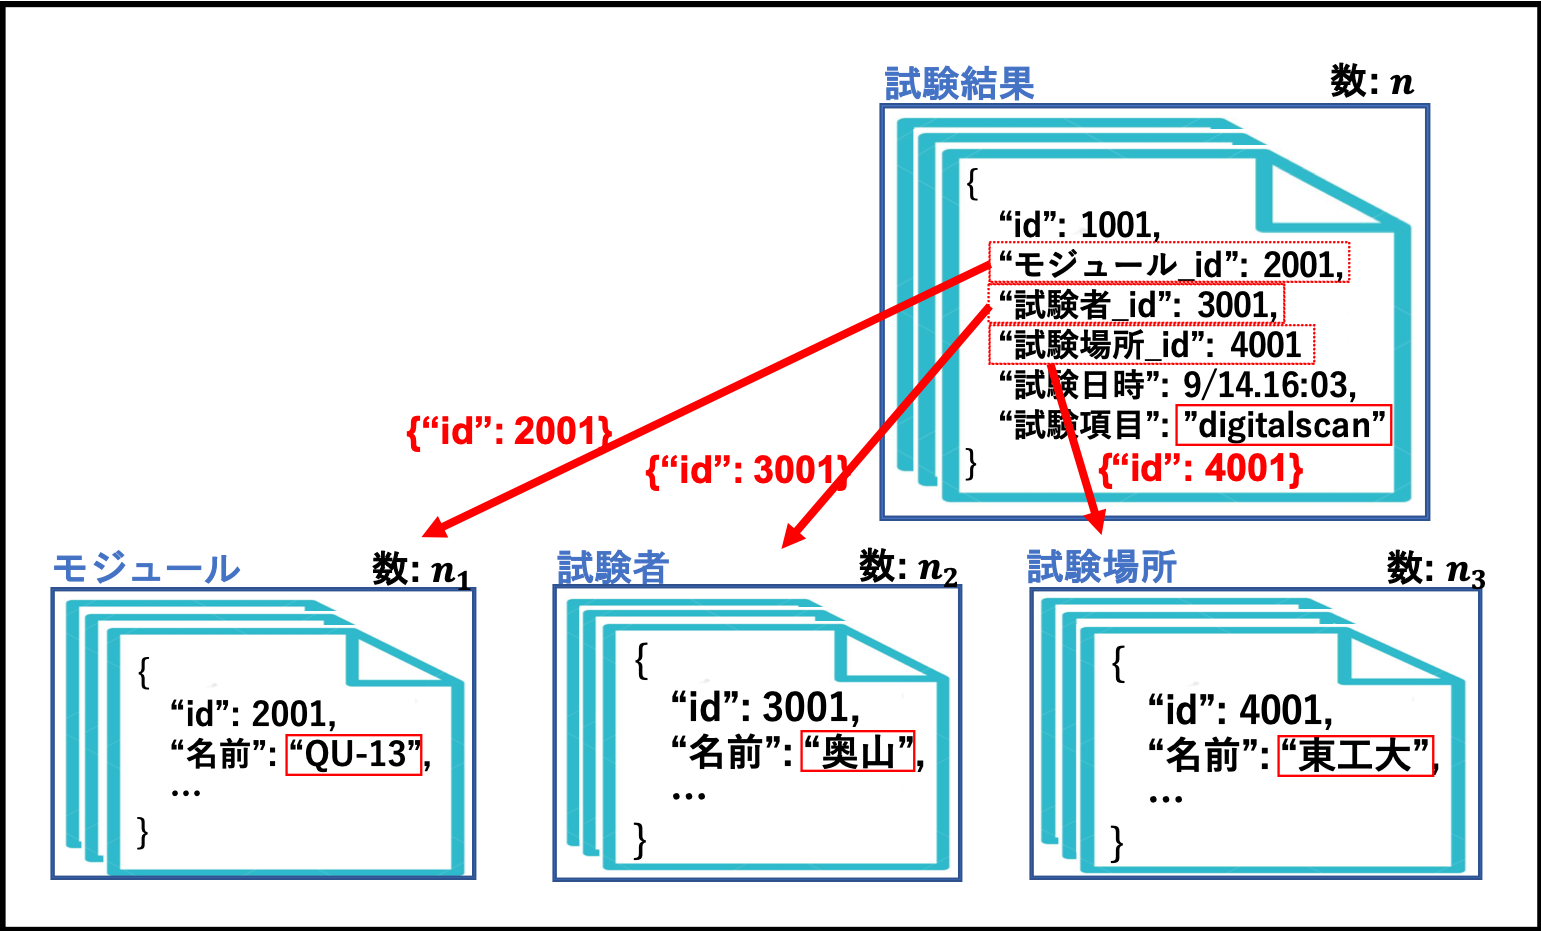
\includegraphics[width=12cm]{search_python_list_problem}
  \caption[検索機能実装方法1の問題点]
{検索機能実装方法1の問題点のイメージ図。図\ref{search_python_list}でも述べたように、検索対象となる情報はこの図のように複数のコレクションにまたがって保存される。そのため、コレクションを超えて検索を行うような場合は試験結果の数以上に、処理に時間がかかってしまう。この図の例の場合、あるコレクション検索にかかる時間がドキュメント数に対して線形とすると、$O(n*(n_1+n_2+n_3))$の処理時間がかかると考えられる。}
  \label{search_python_list_problem}
  \end{center}
\end{figure}

\begin{figure}[bpt]
  \begin{center}
    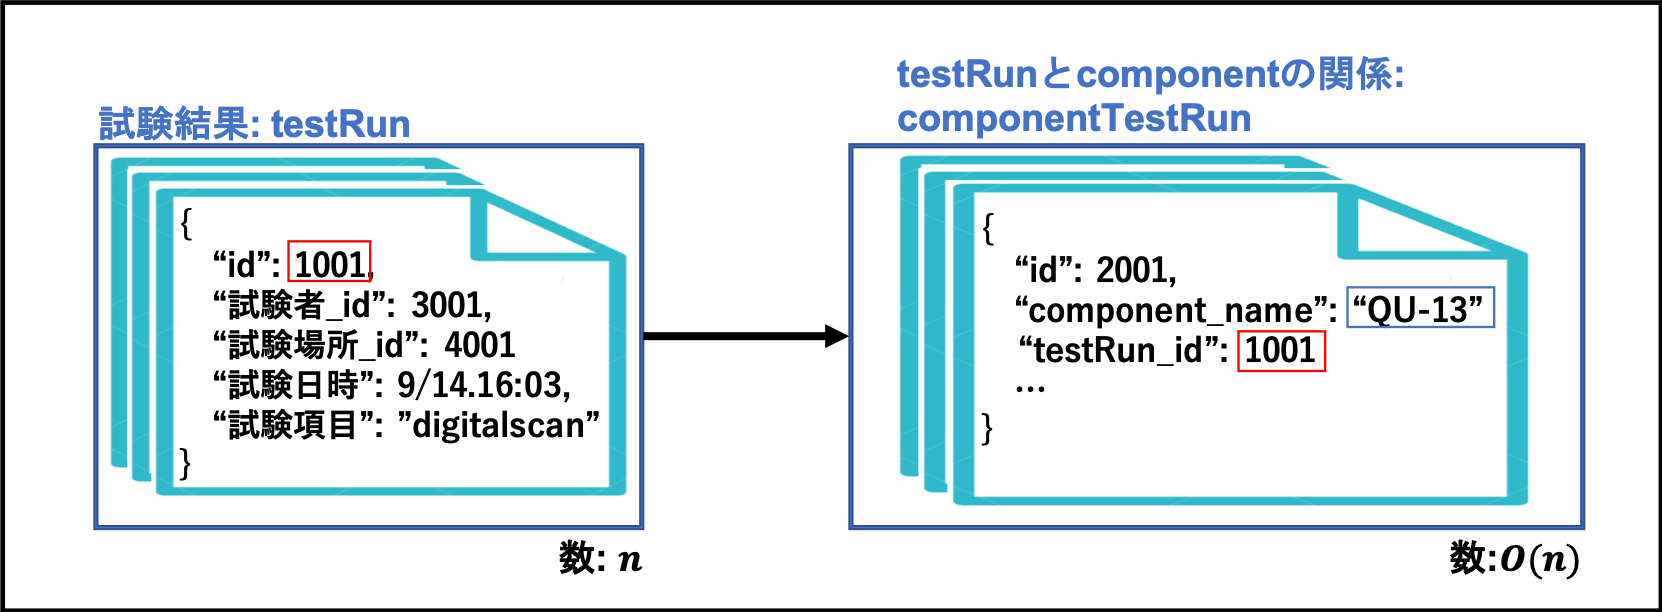
\includegraphics[width=12cm]{search_python_testRun}
  \caption[検索処理時間のボトルネックとなっているデータ構造]{検索処理時間のボトルネックとなっているデータ構造の図。読み出し試験におけるデータ構造(図\ref{localdb_structure_detail})の1つに、各試験結果情報を保存するtestRun、componentとtestRunの関係性を保持するcomponentTestRunという構造が存在する。試験結果数を$n$とすると、testRunのドキュメント数は$n$、componentTestRunの数は試験数とcomponentの数の積となるため$O(n)$となる。結果的に検索処理に$O(n^2)$の時間がかかってしまう。}
  \label{search_python_testRun}
  \end{center}
\end{figure}

\begin{figure}[bpt]
  \begin{center}
    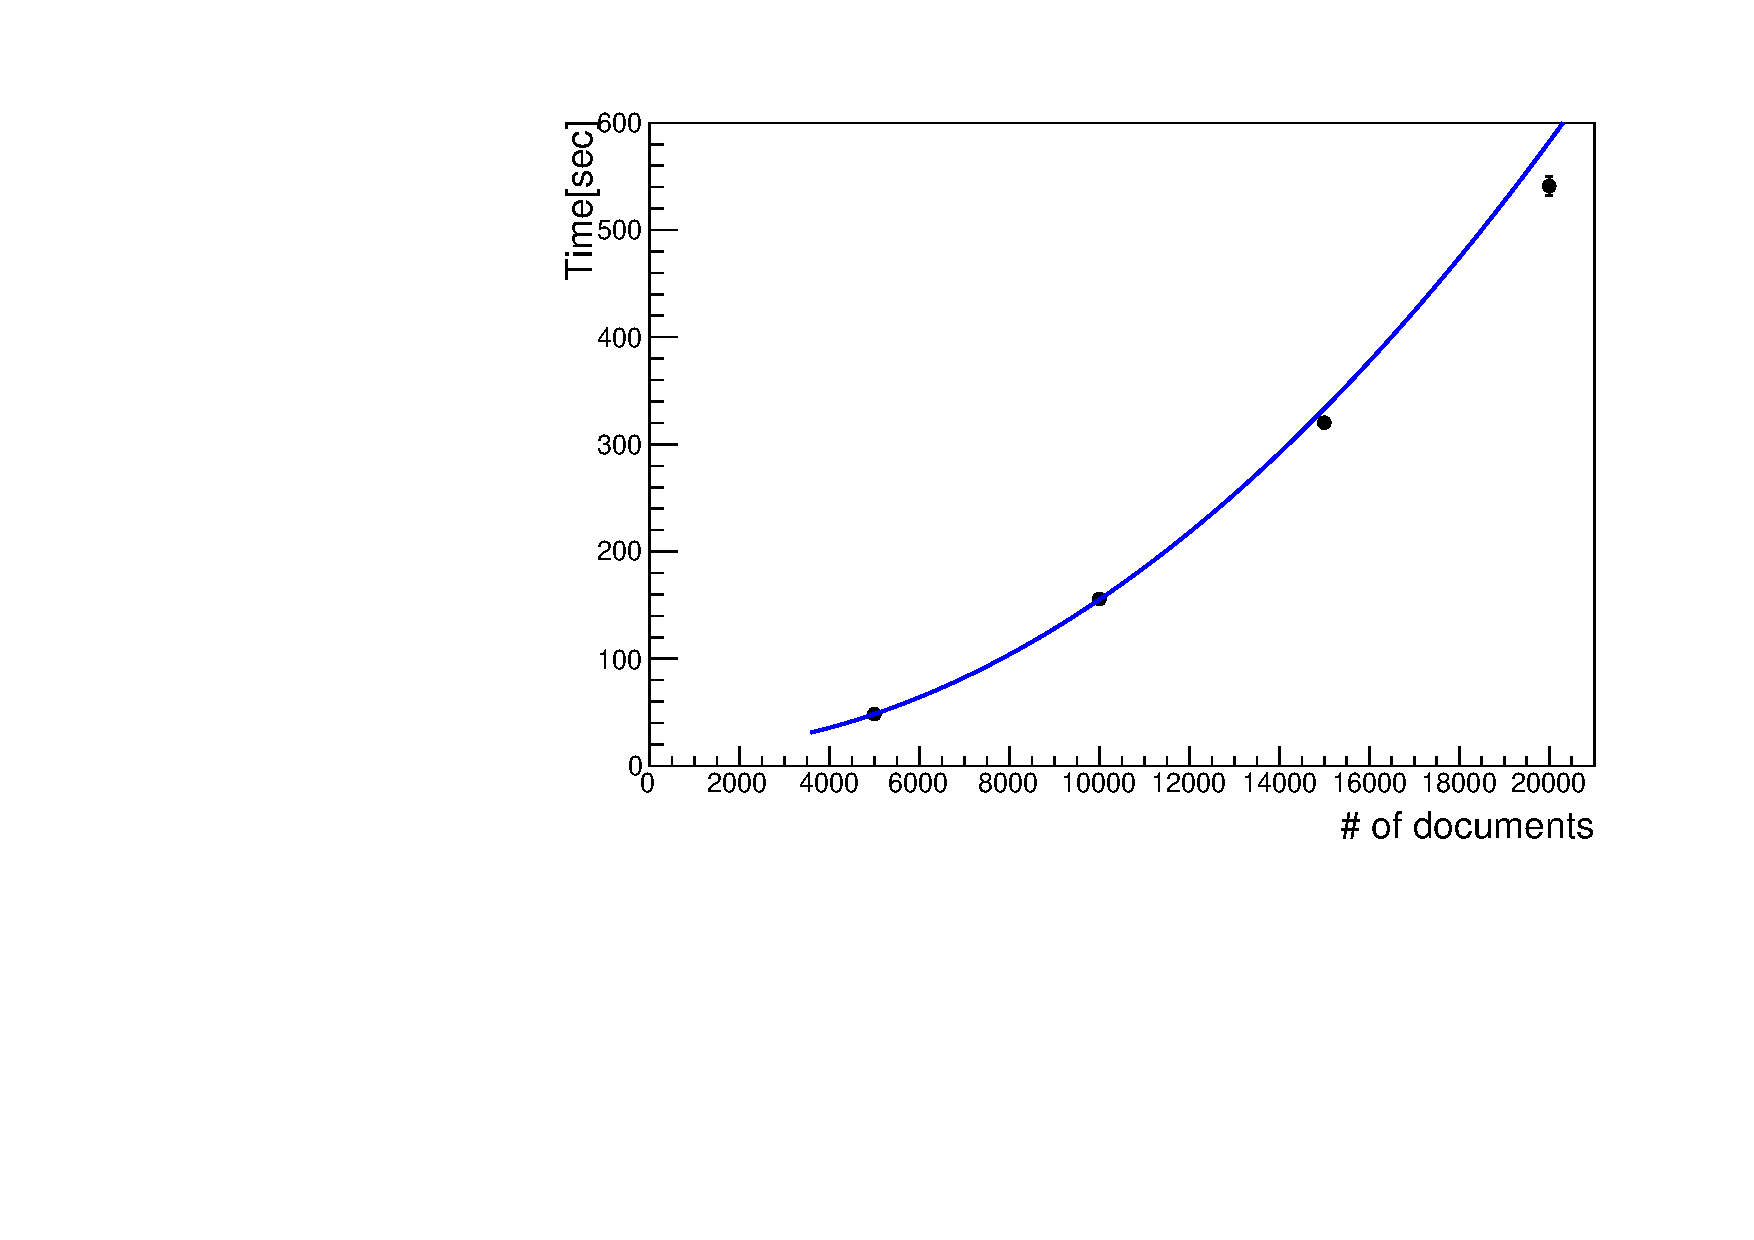
\includegraphics[width=8cm,angle=270]{result_python_list_search.pdf}
  \caption[方法1における検索処理速度測定結果]{方法1における検索処理速度測定結果。横軸が試験結果のドキュメント数、縦軸が処理時間を表している。図\ref{search_python_testRun}で述べたように、方法1の検索処理では試験結果数$n$に対して$O(n^2)$の検索時間がかかため、試験結果のドキュメント数に対して処理時間は二次関数になっていることがわかる。近似関数や生産時における処理時間の見積もりに関しては後述する。}
  \label{searching_time_python_list}
  \end{center}
\end{figure}

%%%%%%%%%%%%%%%%%%%%%%%%%%%%%%%%%%%%%%%%%%%%%%%%%%%%%%%
%%%%%%%%%%%%%%%%%%%%%%%%%%%%%%%%%%%%%%%%%%%%%%%%%%%%%%%

\clearpage
\subsection{方法2: 検索情報を持つドキュメントを作成、使用}

検索機能を改善するため方法2を考案し、実装を行った。
改善の方法として、読み出し試験のアップロードシステム及びウェブアプリケーションでの結果確認システムは既に使われていたため、データ構造及び使用しているPythonフレームワークの変更はせずに処理時間を改善することを試みた。

改善策として、検索キーワードを別のドキュメントに予め保持しておき、処理実行時にはそれを参照することで検索を行う方法を考案し、試験を行った。
アルゴリズムのイメージを図\ref{search_mongo_collection}に示す。
検索情報コレクションに入るドキュメント数は、試験結果数と同じである。
なお、このコレクションはウェブアプリケーションの立ち上げ時に生成するシステムとした。
そのため試験結果数に対する処理時間は$O(n)$と考えられ、方法1に比べて検索コストを削減できると考えた。

\begin{figure}[bpt]
  \begin{center}
    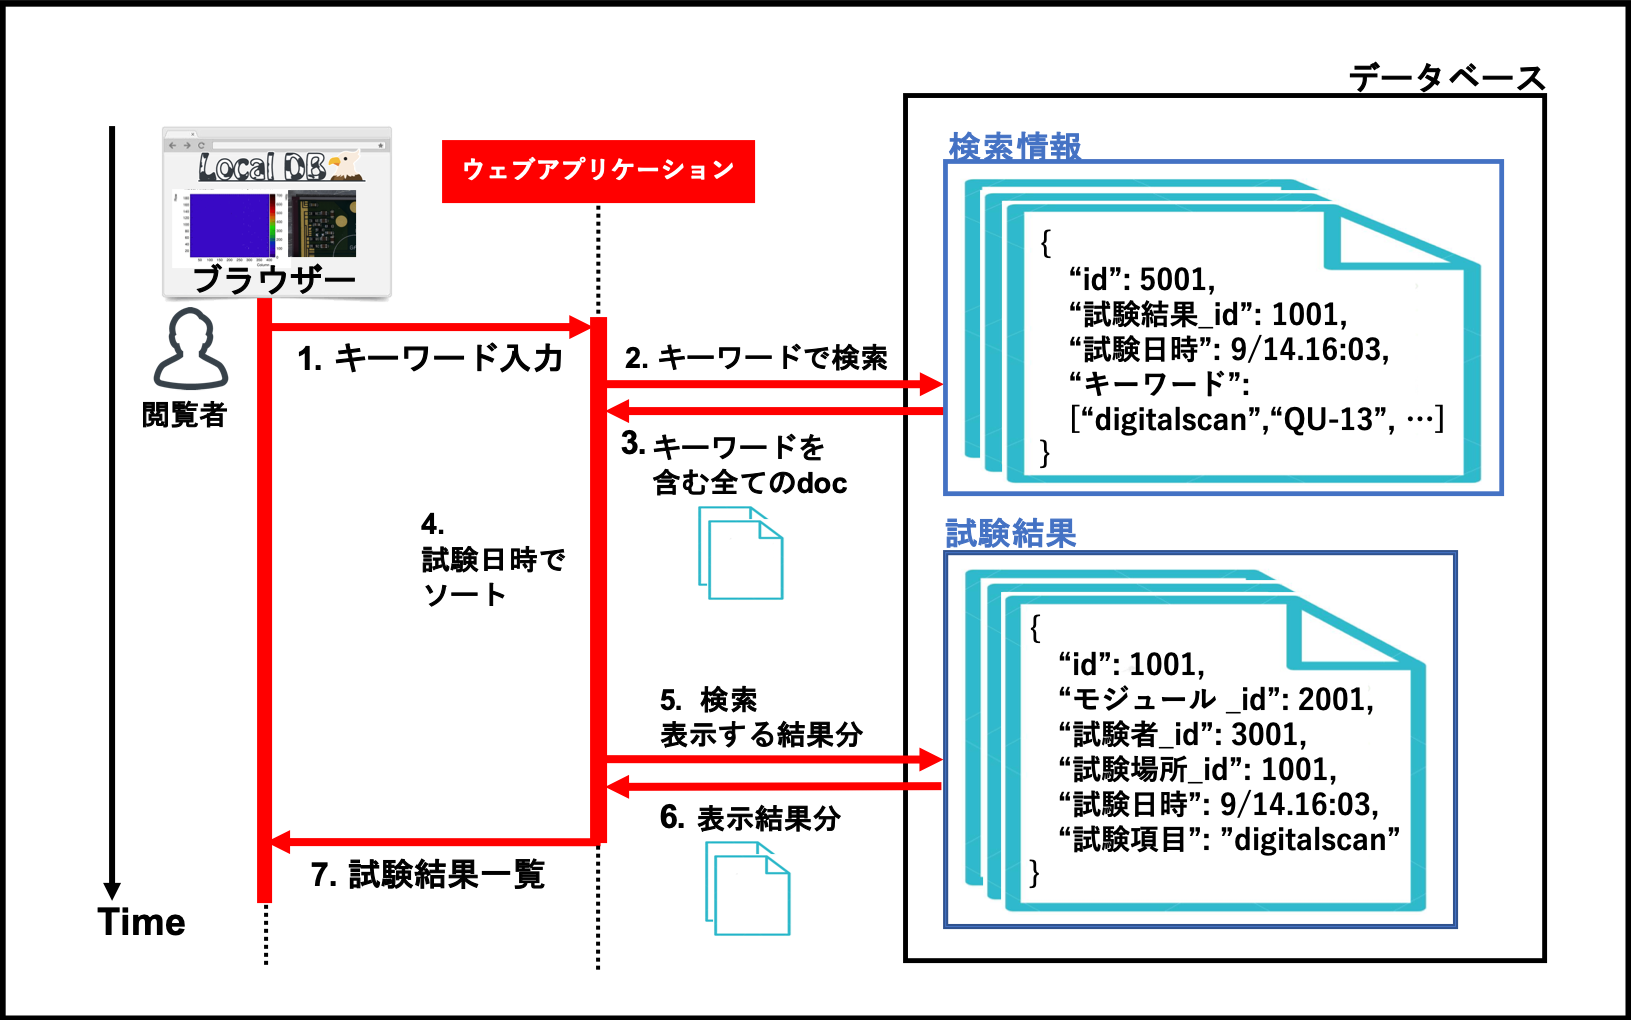
\includegraphics[width=12cm]{search_mongo_collection}
    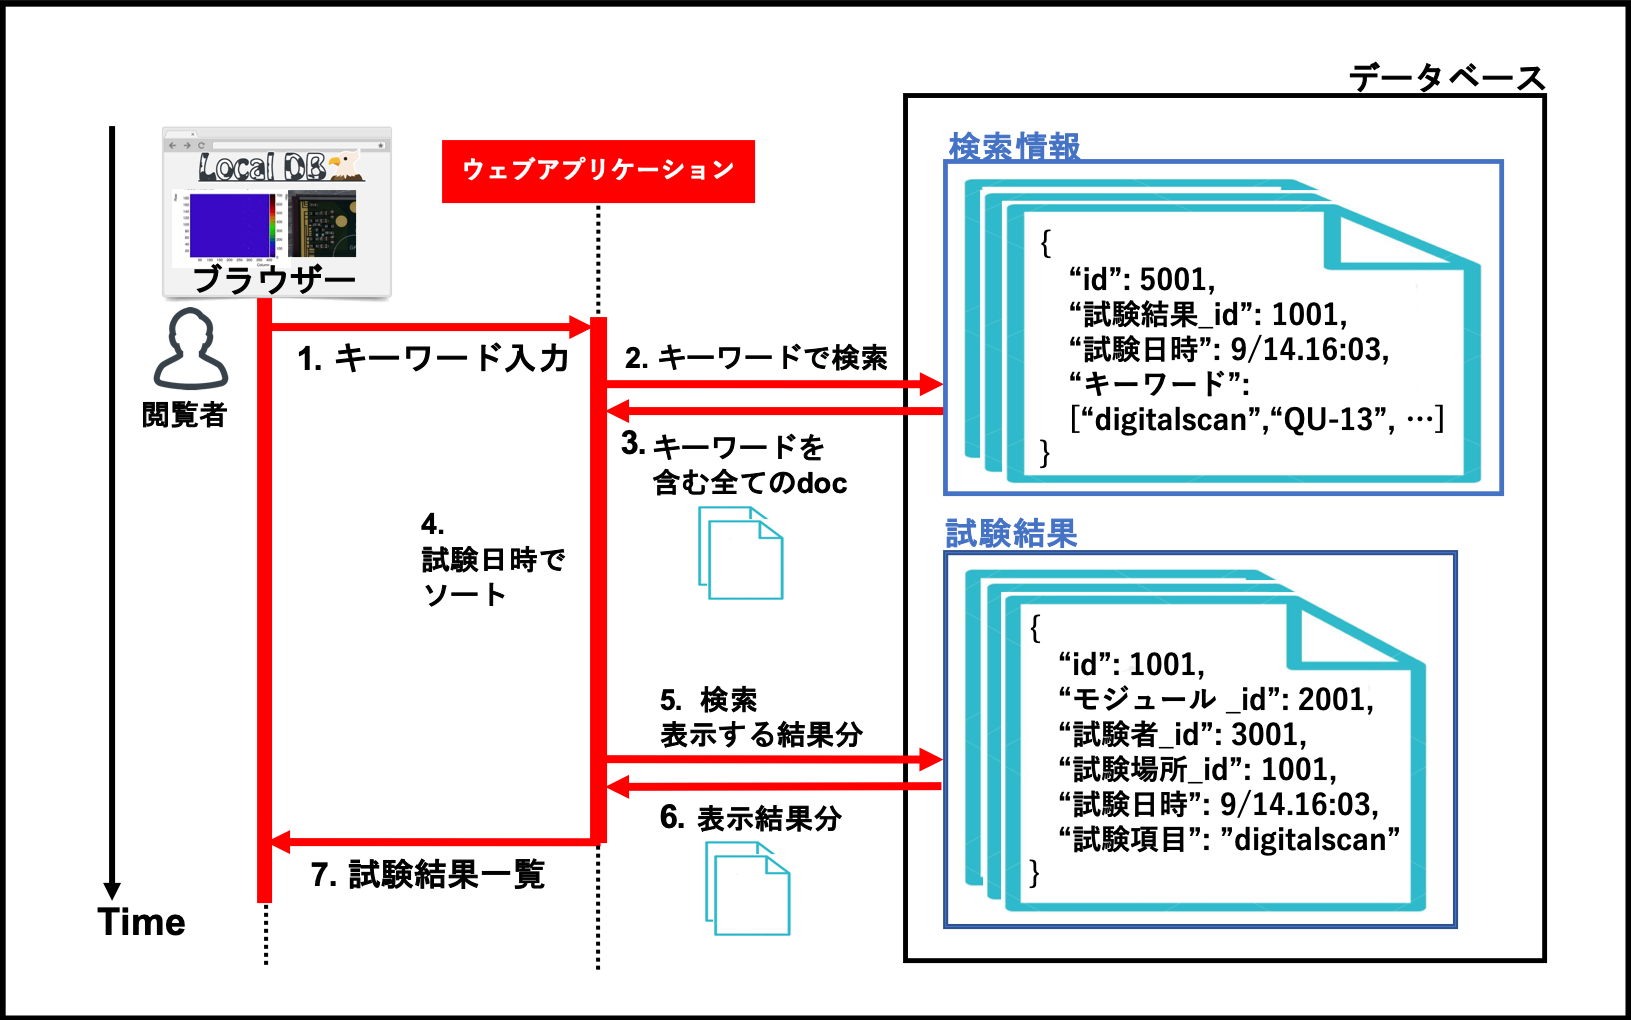
\includegraphics[width=12cm]{search_mongo_collection_flow}
  \caption[検索機能実装方法2:検索キーワード専用コレクションを用いた場合]{検索機能実装方法2:検索キーワード専用コレクションを用いた場合のイメージ図。上図は各コレクションと保存されている情報の例を示しており、下図は実際に検索を行った時の処理の流れを表している。方法2では上図の赤枠で囲っている検索情報のコレクションを新たに設け、これを参照することで検索処理を行う。このコレクション内には各試験結果に対応したドキュメントが1つ保存され、全検索情報と試験結果のIDを持つものとなっている。
処理の流れとしては下図のように、検索情報のコレクションよりキーワードに対応する試験結果を抽出する処理と、表示の際に必要な情報を試験結果のコレクションから取得する処理の2つに分かれた構造となっている。
このような処理をすることにより、各検索処理にかかる時間は試験結果数に対して$O(n)$になると考えられる。}
  \label{search_mongo_collection}
  \end{center}
\end{figure}

以下に検索情報のドキュメントの例をリスト\ref{example_doc_searchhash}に示す。
\begin{lstlisting}[basicstyle=\scriptsize,caption=検索情報コレクションに入るドキュメントの例。このように試験結果のID、試験日時、検索対象となる名前情報が保存される。,label=example_doc_searchhash]
{
	"_id" : ObjectId("5fd489f60e2ca70557e44a8b"),
	"runId" : "5fc4d027b1ef7c6297c91040",
	"timeStamp" : ISODate("2020-11-30T10:57:19Z"),
	"data" : [
		"20UPGR00000001",
		"20UPGFC9999999",
		"std_digitalscan",
		"hokuyama",
		"tokyo_institute_of_technology",
		"2020/12/09"
	]
}
\end{lstlisting}

%%%%%%%%%%%%%%%%%%%%%%%%%%%%%%%%%%%%%%%%%%%%%%%%%%%%%%%
%%%%%%%%%%%%%%%%%%%%%%%%%%%%%%%%%%%%%%%%%%%%%%%%%%%%%%%

\clearpage
\section{処理時間測定} \label{sec:search_process_time_mes}

考案した方法を実装し、検索処理時間の測定を行った。詳細を以下に示す。
また方法1において行った処理時間測定も同様の条件で行った。

\subsubsection{使用した装置}

測定には個人的に使用しているノートPC(MacBookAir(13-inch,2017))を用いた。
性能を表\ref{laptop_spec}に示す。

\begin{table}[tbp]
\caption[測定に使用したノートPCの性能]{測定に使用したノートPC(MacBookAir(13-inch,2017))の性能。検索処理時間の測定に個人的に使用しているノートPCを使用した。}
\label{laptop_spec}
\scalebox{0.9}{
  \begin{tabular}{|l|llll|l|l|} \hline
    種類 & CPU & & & & Memory & Disk \\
     & Type & Core & Thread & Clock speed[GHz]& [GB] & [GB] \\ \hline 
    MacBookAir(13-inch,2017) & Intel Core i5 & 2 & 4 & 1.8 & 8 & 256\\ \hline
  \end{tabular}
}
\end{table}

\subsubsection{測定内容}

コマンドプロンプトから以下のコマンドを実行し、ある試験結果ページのリクエストに対するアプリケーションのレスポンス時間を測定した。
ここでは検索キーワードは"okuyama"とし、検索モードは部分一致としている。
実際にアプリケーションを使用する際には、ブラウザーに一覧表示をする時間が今回の測定時間に加算されることになる。

{ \small
\begin{lstlisting}
curl "http://127.0.0.1:5000/localdb/scan?keywords=okuyama&match=partial" 
-o /dev/null -w "\%{time\_total}\n" 2> /dev/null -s
\end{lstlisting}
}

その他測定に関する詳細を表\ref{searching_measurement_details}に示す。

\begin{table}[tbp]
\begin{center}
\caption[検索機能処理時間測定の詳細]{検索機能処理時間測定の詳細。測定を行った試験結果数、回数、キーワード、検索モード、検索情報の詳細を示している。}
\label{searching_measurement_details}
\scalebox{0.9}{
  \begin{tabular}{|l|l|} \hline
    試験結果数 & 5000, 10000, 15000, 20000\\
    測定回数 & 各測定点に対して20回\\
    検索キーワード & okuyama\\
    検索モード & 部分一致\\
    各試験結果が持つ検索情報 & 全試験結果に対して同じ、以下に詳細\\\hline
    検索情報一覧             & モジュール名: 20UPGR10000005\\
		                         & FEチップ名:   20UPGTU9000000\\
		                         & 試験項目:     std$\_$digitalscan\\
		                         & 試験者:       okuyama\\
		                         & 試験場所:     default$\_$host\\
		                         & 試験日時:     2020/12/06\\\hline
  \end{tabular}
}
\end{center}
\end{table}

各測定点に対して平均値、標準偏差を算出し、フィッティングを行った。

\subsubsection{測定結果}

方法2を用いて得られた結果を図\ref{searching_time}に示す。
また方法1の結果に関しては、既に図\ref{searching_time_python_list}で示した。
方法1、方法2で得られた近似関数を式\ref{function_python_list}、\ref{function_mongo_collection}に示す。
方法1に対して、方法2はアルゴリズムの改善が見られる。

\begin{figure}[bpt]
  \begin{center}
  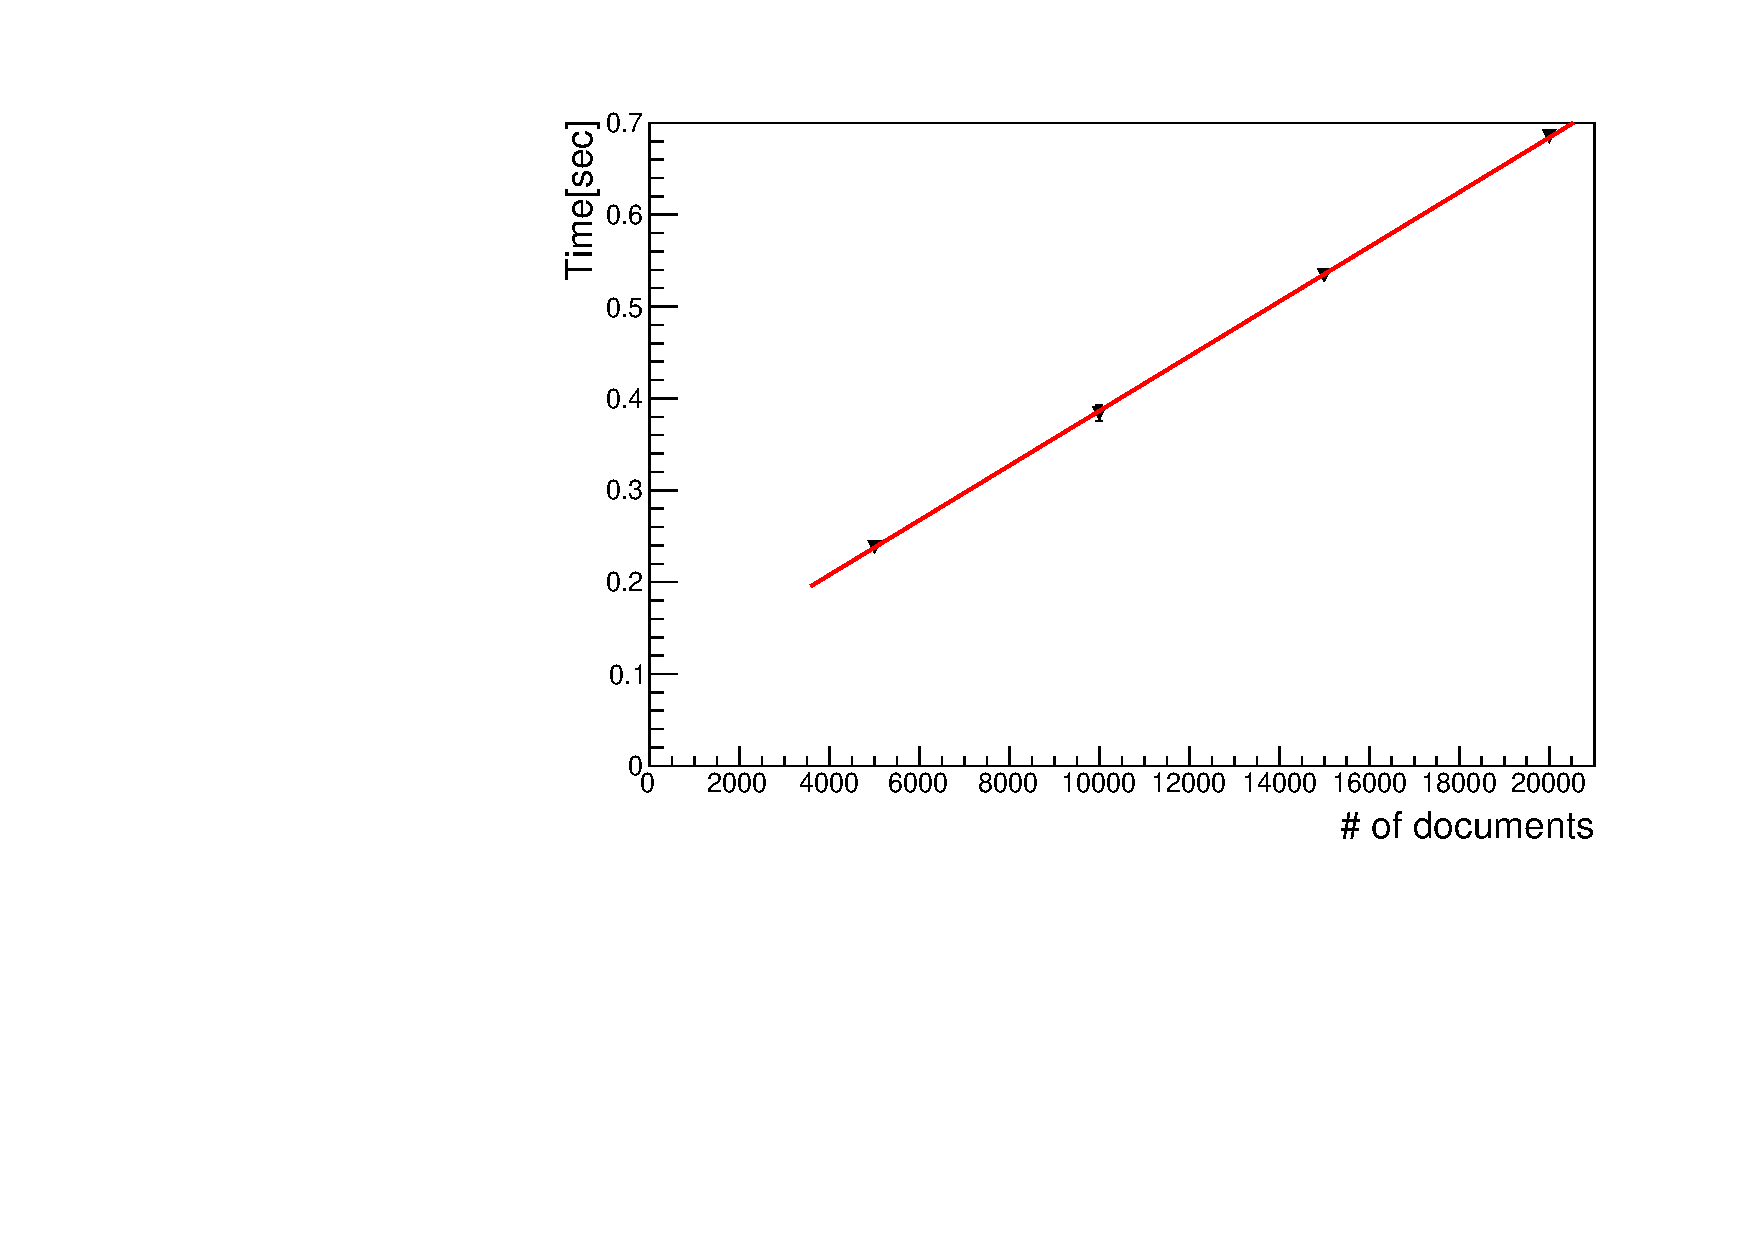
\includegraphics[width=8cm,angle=270]{result_mongo_collection_search.pdf}
  \caption[方法2における検索処理時間測定結果]{方法2における検索処理時間測定結果。横軸が試験結果のドキュメント数、縦軸が処理時間を表している。線形性を示していることが確認でき、検索実行時における処理時間は方法1に比べて優れている。}
  \label{searching_time}
  \end{center}
\end{figure}

\bbb
y &=&  ax^2 + b \\
\label{function_python_list}
a &=& (1.4\pm0.0)\times10^{-6} \nonumber \\
b &=& 13\pm 0 \nonumber
\eee

\bbb
y &=& ax + b \\
\label{function_mongo_collection}
a &=& (3.0\pm0.1)\times10^{-5} \nonumber \\
b &=& (8.9\pm 0.8)\times10^{-2} \nonumber
\eee

現在は方法2で検索機能を実装し、サービスの1つとして提供している。


方法2では、アプリケーションの起動時に検索情報コレクションを生成するアルゴリズムとしている。
ここで検索情報コレクションの生成にかかる処理時間として、ドキュメント数に対するアプリケーションの起動時間を測定した。
結果を図\ref{creating_cache_time}に示す。
基本的には方法1と同じ操作を行うことで検索情報を収集し、ドキュメントを作成する。
そのため、処理時間は$O(n^2)$となる。
この処理を前もって行なうことで、検索実行時の処理性能を上げている。
\begin{figure}[bpt]
  \begin{center}
  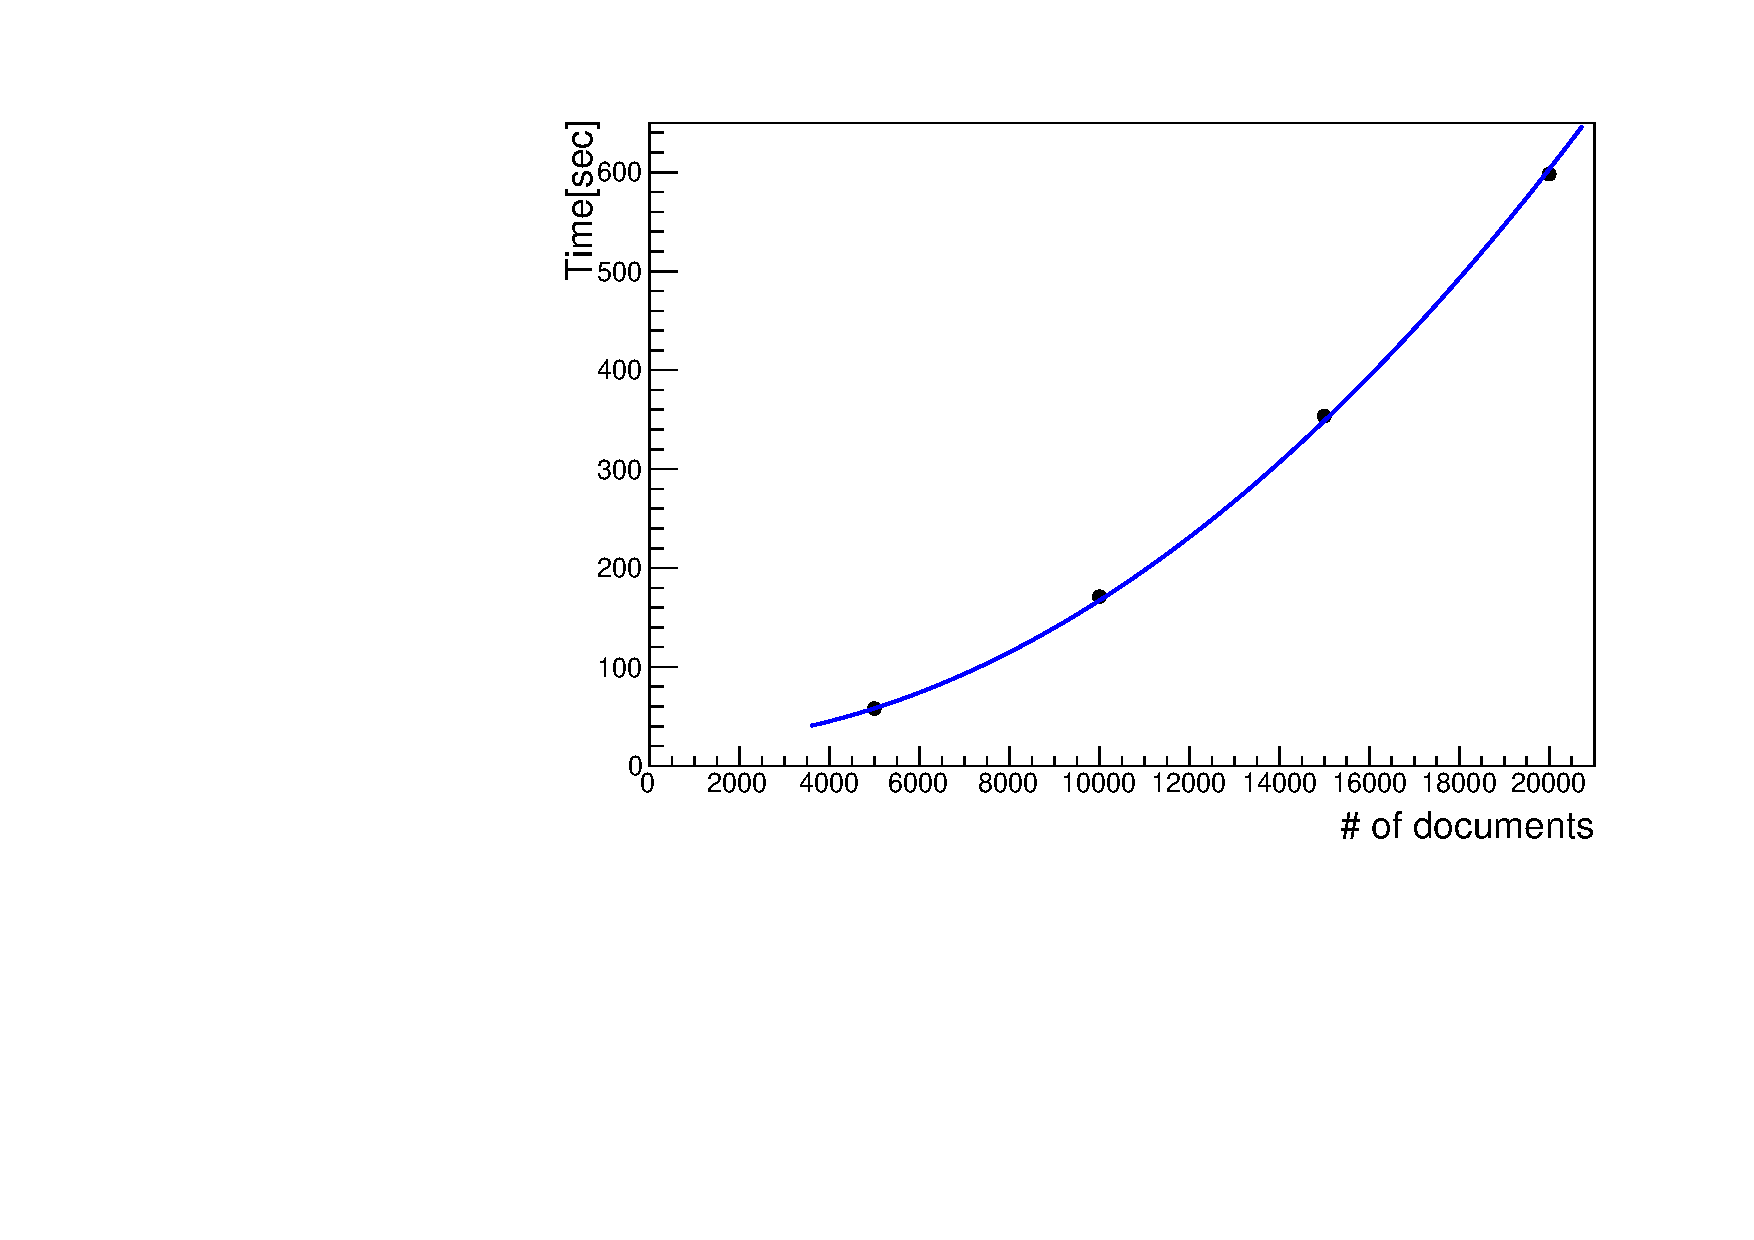
\includegraphics[width=8cm,angle=270]{creating_cache_time.pdf}
  \caption[方法2における検索情報コレクションの生成時間測定結果]{方法2における検索情報コレクションの生成時間測定結果。検索情報コレクションの生成にかかる処理時間として、ドキュメント数に対するアプリケーションの起動時間を測定した。横軸が試験結果のドキュメント数、縦軸が時間を示している。検索情報コレクションの生成には、方法1と同様の処理を行なっているため$O(n^2)$となっているのが分かる。}
  \label{creating_cache_time}
  \end{center}
\end{figure}

\subsubsection{生産時における検索時間の見積もり}
各方法について、生産時における処理時間の見積もりを行う。簡単のため今回使用したデバイスと生産時に使うサーバーの性能差は無視する。
ここでデータベースで管理するモジュール数は日本が最多とし、その数を予定している2,000とする。
保存する読み出し試験数は3章で述べたように、1つのモジュールあたり42とする。全ての生産が終了した際の検索処理時間を見積もる。
上で得られた関係式を用いて検索処理実行時間は方法1、2に対して式\ref{estimated_python_list}、\ref{estimated_mongo_collection}のように見積もることができる。

\bbb
\{(1.4\pm0.0)\times10^{-6}\}\times(2000\times42)^2 + (13\pm 0) = (9.8\pm0)\times10^{3} [\rm{sec}]
\label{estimated_python_list}
\eee
\bbb
\{(3.0\pm0.1)\times10^{-5}\}\times(2000\times42) + \{(8.9\pm 0.8)\times10^{-2}\} = 2.6\pm0.1 [\rm{sec}]
\label{estimated_mongo_collection}
\eee

方法1では1回の検索に対して約2.7時間と見積もられ、生産時には検索機能として運用不可能なシステムであることがわかる。
方法2では終了時点においても数秒で処理を終えることができるため、生産を通して十分に使うことができると考えられる。
 

%%%%%%%%%%%%%%%%%%%%%%%%%%%%%%%%%%%%%%%%%%%%%%%%%%%%%%%%%%%%%%%%%%
%%%%%%%%%%%%%%%%%%%%%%%%%%%%%%%%%%%%%%%%%%%%%%%%%%%%%%%%%%%%%%%%%%

\clearpage
\section{改善方法の処理時間測定}
より処理時間を短くすることを目的として、新たな検索処理アルゴリズムの考案と測定を行った。詳細について以下に示す。

\subsection{方法2における検索処理時間の詳細調査}
先述したように、方法2では処理時間が改善した。
この方法2について、処理時間の詳細を知るために追加で測定を行った。
アプリケーション層での各処理について、以下のように番号をつける。
\begin{enumerate}
  \item キーワードを受け取り、検索情報コレクションに検索をかけるまでの処理.
  \item 検索情報コレクションに検索をかけ、情報を受け取る処理.
  \item ドキュメントを受け取り該当する試験結果IDをまとめ、試験結果に対して検索をかけるまでの処理.
  \item 試験結果コレクションに検索をかけ、情報を受け取る処理.
  \item ドキュメントを受け取りデータを整形、ブラウザにレスポンスを返すまでの処理.
\end{enumerate}

イメージを図\ref{search_mongo_collection_details}に示す。

\begin{figure}[bpt]
  \begin{center}
    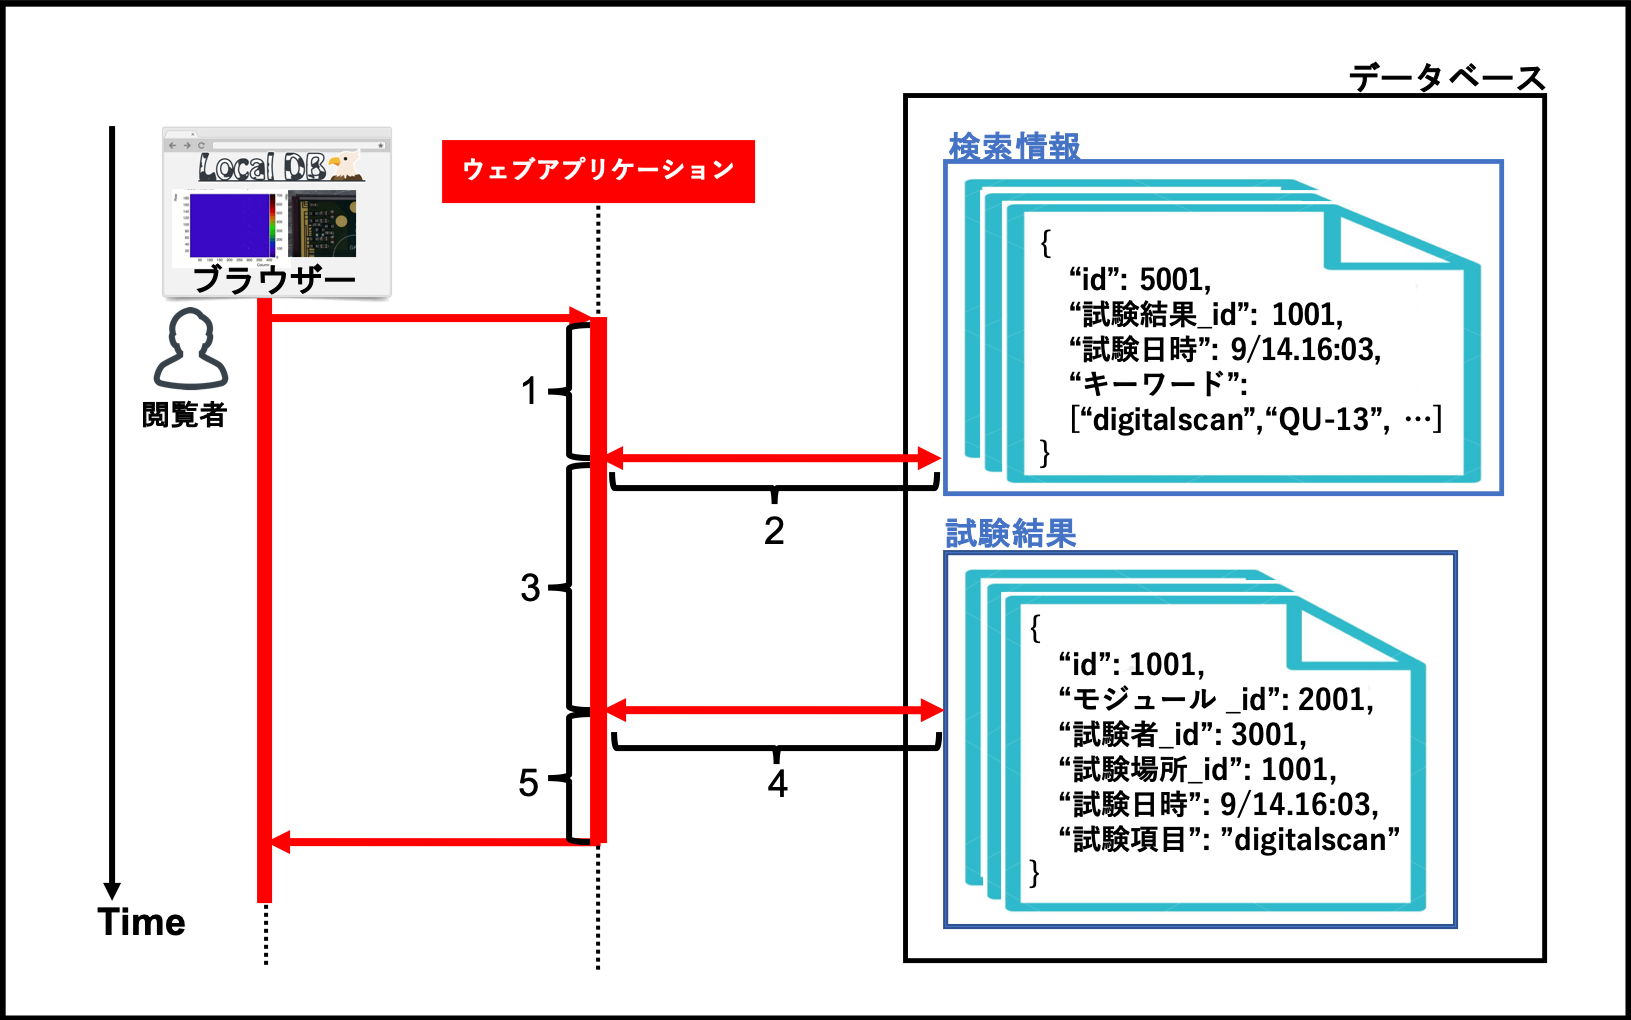
\includegraphics[width=12cm]{search_mongo_collection_details}
  \caption[方法2の検索における詳細処理]{方法2の検索における詳細処理。図のように全体の流れにおけるアプリケーション内部での各処理、データベースから情報取得の各処理に1から5の番号をつけそれぞれにかかる処理時間を測定した。}
  \label{search_mongo_collection_details}
  \end{center}
\end{figure}

ボトルネックとなっている処理を測定するために、上述した各処理にかかる時間の測定を行った。
測定は試験結果数が10,000の場合に行った。また測定は20回行った。

結果を図\ref{search_mongo_collection_details_result}に示す。

\begin{figure}[bpt]
  \begin{center}
    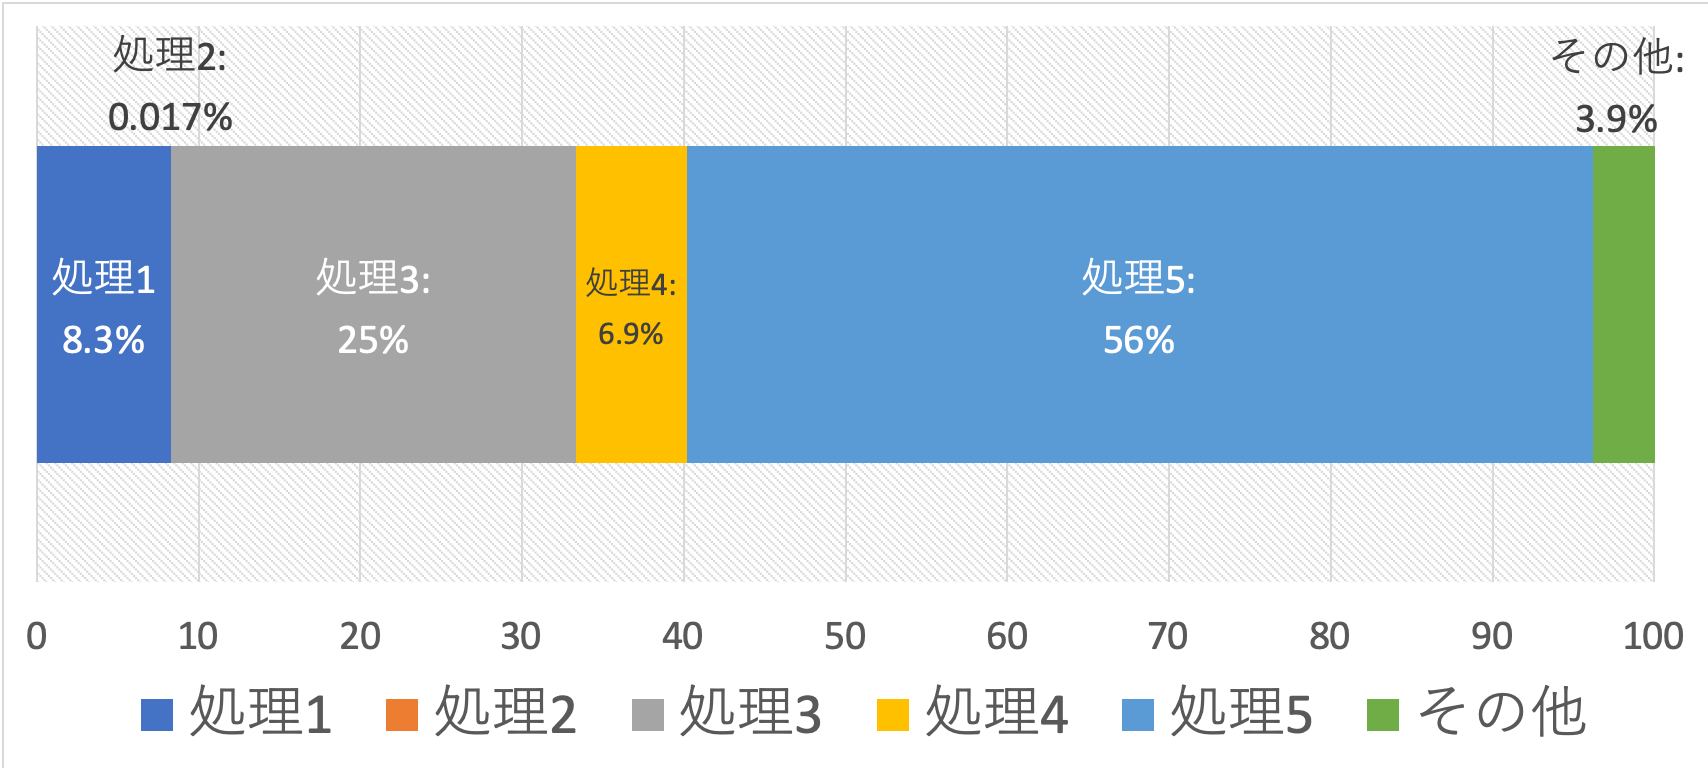
\includegraphics[width=12cm]{search_mongo_collection_details_result}
  \caption[方法2における詳細処理時間の測定結果]{方法2における詳細処理時間の測定結果。図\ref{search_mongo_collection_details}における5つの詳細処理にかかる時間の割合を表している。処理3、5にあたるコレクション検索実行後のアプリケーション内での処理に多く時間がかかっていることが分かる。}
  \label{search_mongo_collection_details_result}
  \end{center}
\end{figure}

図より処理3、5の割合が大きいことがわかる。
これらの処理について、特に以下の処理の割合が大きいことがわかった。
\bbb
\begin{split}
&取得した複数ドキュメントから\rm{Python}リストへの型変換&
\label{dominated_process}
\end{split}
\eee

図\ref{search_mongo_collection_details}における処理3、5において、型変換処理\ref{dominated_process}の割合を表\ref{ratio_dominated_process}まとめた

\begin{table}[tbp]
\begin{center}
\caption[処理3,5における型変換処理\ref{dominated_process}の割合]{処理3,5における型変換処理\ref{dominated_process}の割合。処理3、5について、表の割合より、型変換処理\ref{dominated_process}が支配的であることが分かる。}
\label{ratio_dominated_process}
\scalebox{1.0}{
  \begin{tabular}{|llll|} \hline
    処理 & 全体[sec] & 処理\ref{dominated_process}[sec] & 割合[$\%$]\\\hline
    3    & 0.091 $\pm$ 0.011 & 0.089 $\pm$ 0.005 & 97 $\pm$ 0  \\
    5    & 0.21 $\pm$ 0.00 & 0.18 $\pm$ 0.00 & 86 $\pm$ 1 \\\hline
  \end{tabular}
}
\end{center}
\end{table}

この変換処理について、あるコレクションにおける全ドキュメント数に対するPythonリスト変換処理時間の関係を測定した。
結果を図\ref{dominated_process_relation}に示す。
全ドキュメント数に対して線形性を示していることがわかる。
方法2の検索処理については処理\ref{dominated_process}が支配的であることが分かった。
\begin{figure}[bpt]
  \begin{center}
    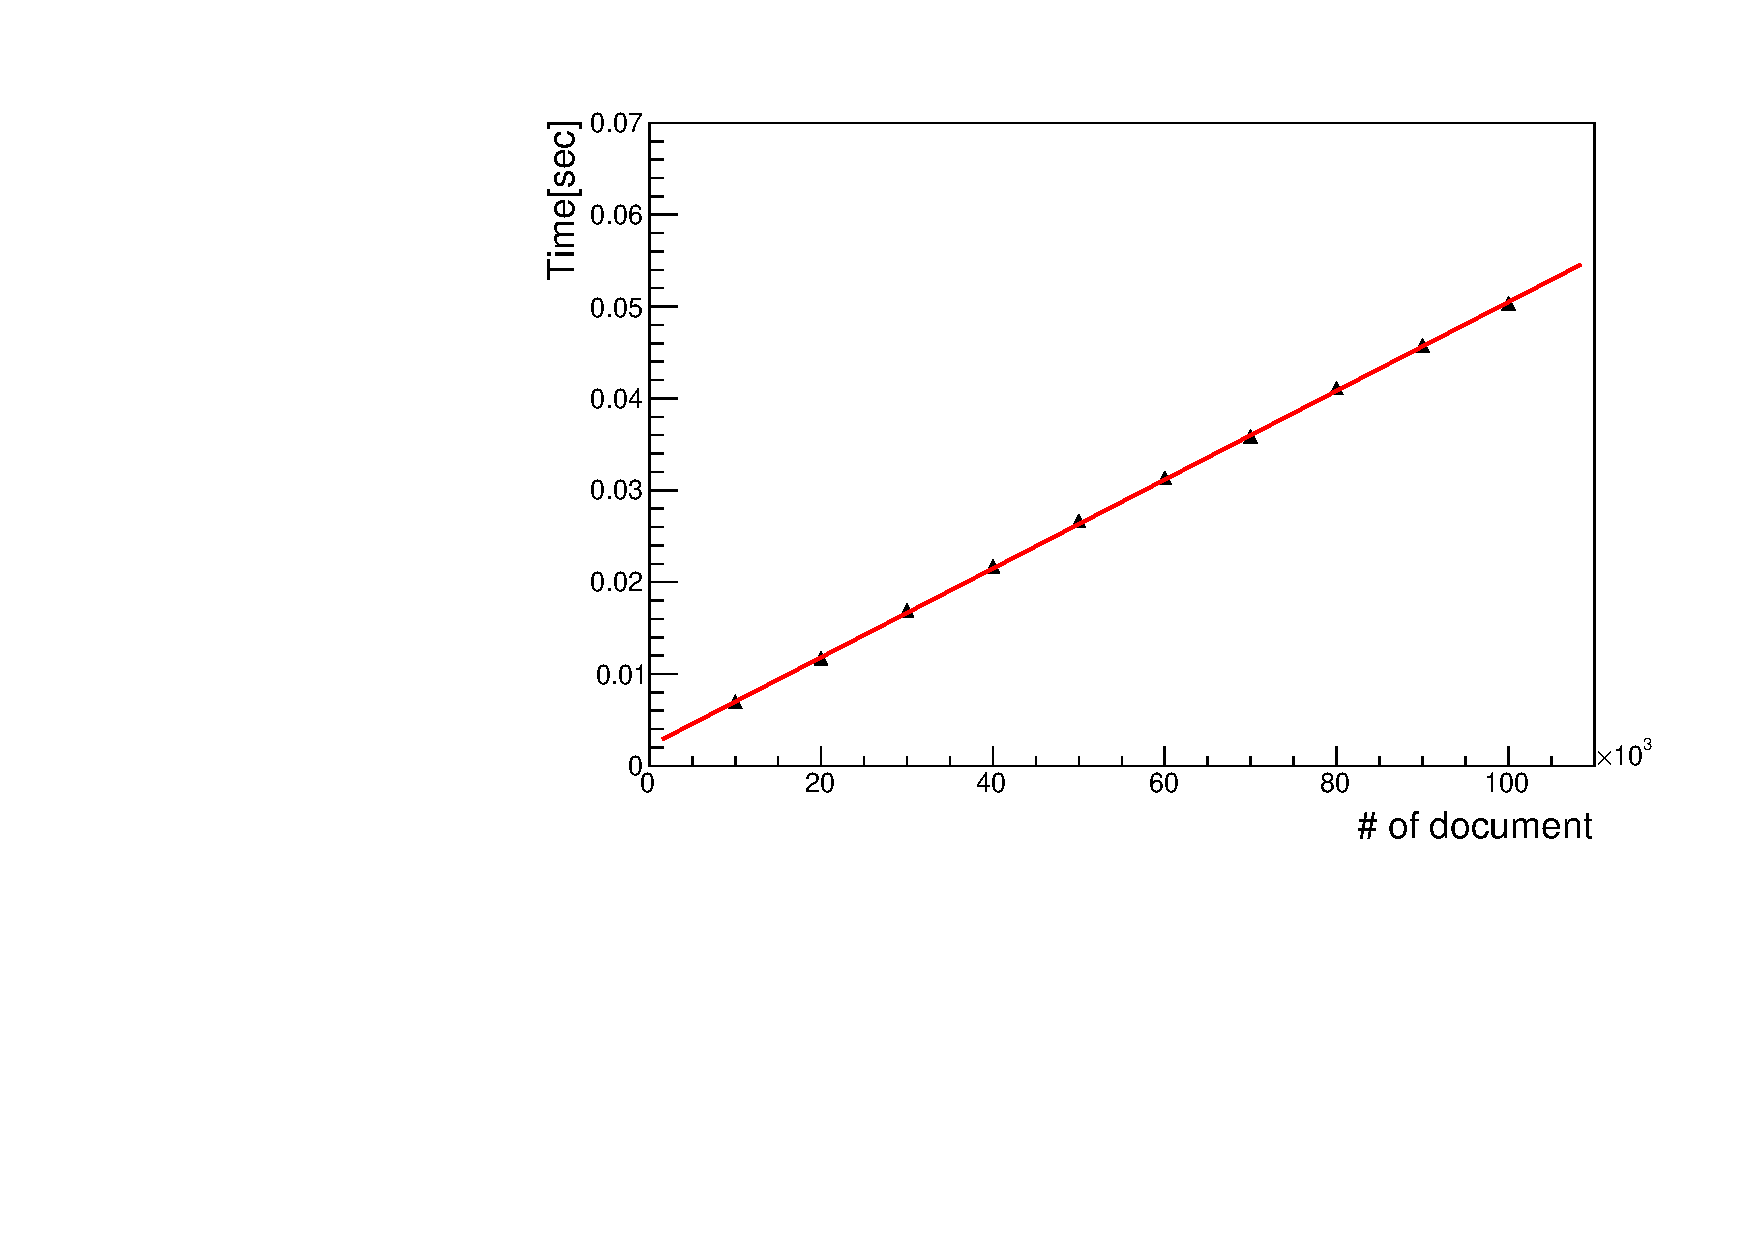
\includegraphics[width=8cm,angle=270]{dominated_process_relation.pdf}
  \caption[ドキュメント数に対する型変換処理時間の関係]{ドキュメント数に対する型変換処理時間の関係。コレクション検索後の型変換に要する処理時間は、図のようにドキュメント数に対して線形となっていることが分かる。}
  \label{dominated_process_relation}
  \end{center}
\end{figure}

\subsection{改善点}

測定を踏まえ、改善方法として以下の項目を検討した。
ここでは、上述したように使用しているデータ構造やフレームワークの変更はせずに処理時間を改善することを前提としている。
\begin{itemize}
  \item コレクション検索処理の回数を減らす.
  \item 検索対象コレクションのドキュメント数を減らす.
\end{itemize}

上述した2つを目的として、以下の2つの方法を新しく考え処理時間測定を行った。

\begin{enumerate}
  \setcounter{enumi}{2}
  \item 検索情報のコレクションに一覧表示に必要な情報を保持、参照.
  \item 方法3に付け加えて、検索情報のドキュメントを複数コレクションに分散、マルチスレッドを用いた検索処理の並列化.
\end{enumerate}

方法3については一覧表示に必要な情報を検索情報のドキュメントが持つことで、データベースに対する検索の回数を減らすことを目的としている。
方法4については方法3の検索処理の数を減らすことに加えて、ドキュメントの数を分散し並列処理をすることで処理時間の改善を図っている。
イメージをそれぞれ図\ref{search_summary_hash}、\ref{search_multi_thread}に示す。

\begin{figure}[bpt]
  \begin{center}
    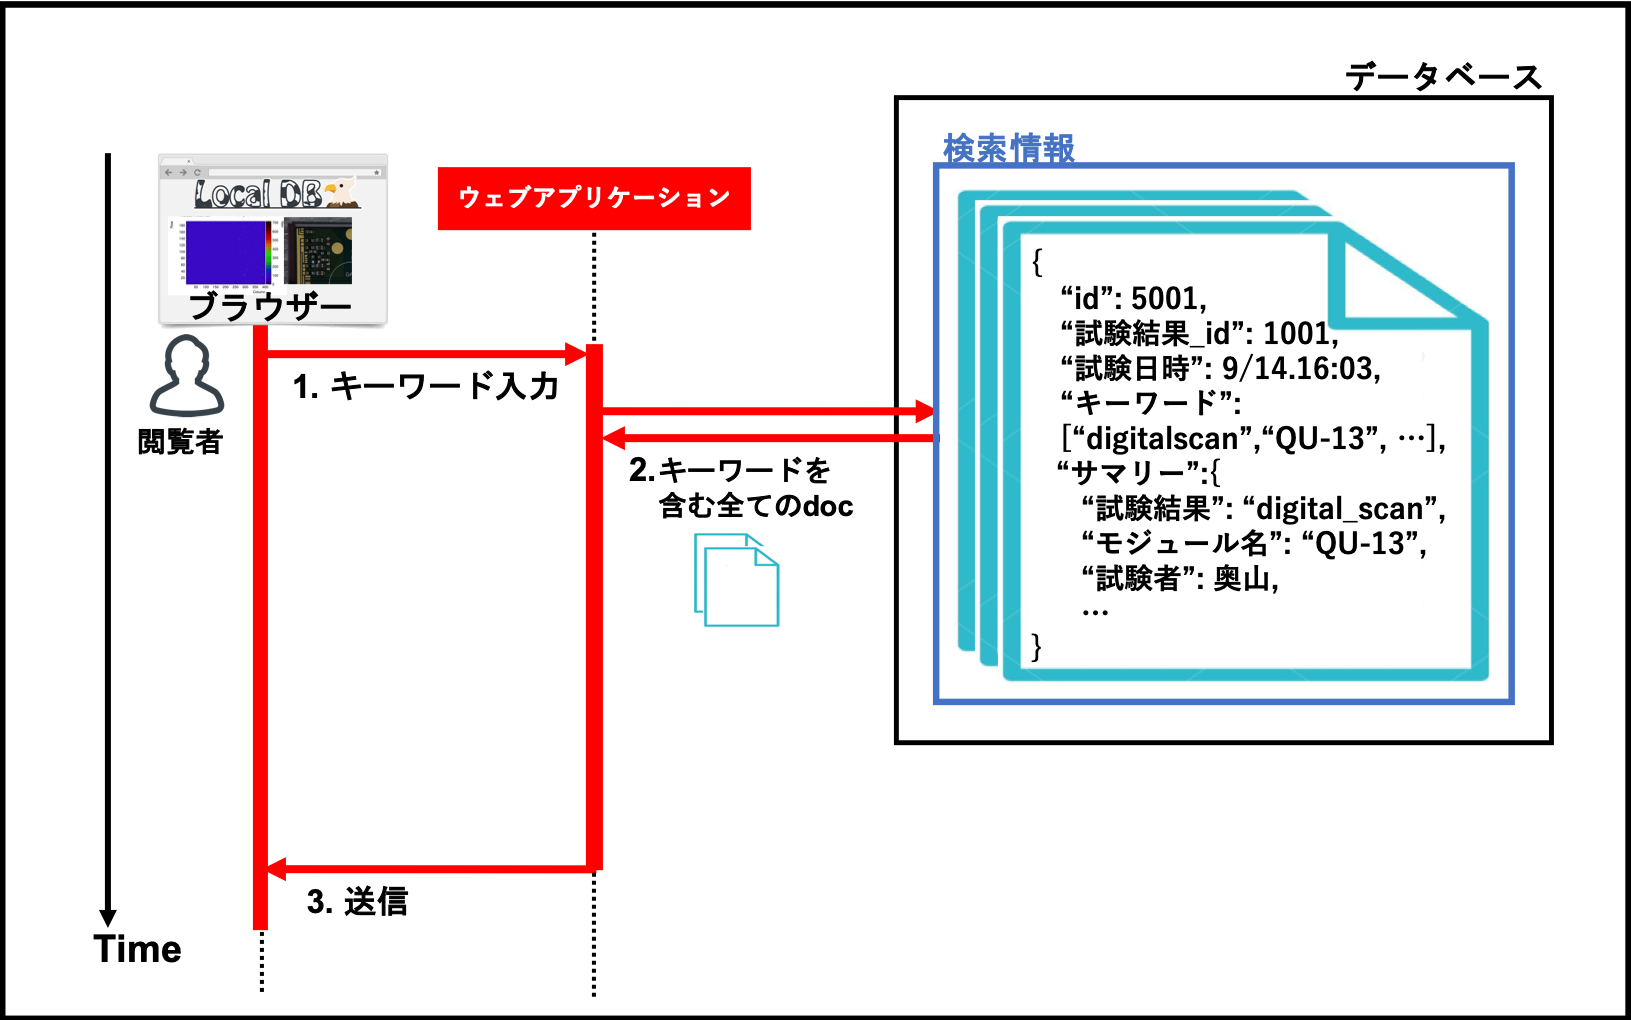
\includegraphics[width=12cm]{search_summary_hash}
  \caption[検索機能実装方法3:検索情報と共に一覧表示に必要な情報を保持、参照]{検索機能実装方法3:検索情報と共に一覧表示に必要な情報を保持、参照。方法2では検索情報コレクションより、条件に一致する試験結果IDを取得し、実際の試験結果に対して再度検索をかける流れとなっていたが、この方法では一覧表示に必要な情報も全て検索情報のコレクション内で保持する。こうすることで検索機能において必要な情報の全てが1つのコレクションにまとまり、コレクション検索の処理が1回で済むため、処理時間が改善すると考えられる。}
  \label{search_summary_hash}
  \end{center}
\end{figure}

\begin{figure}[bpt]
  \begin{center}
    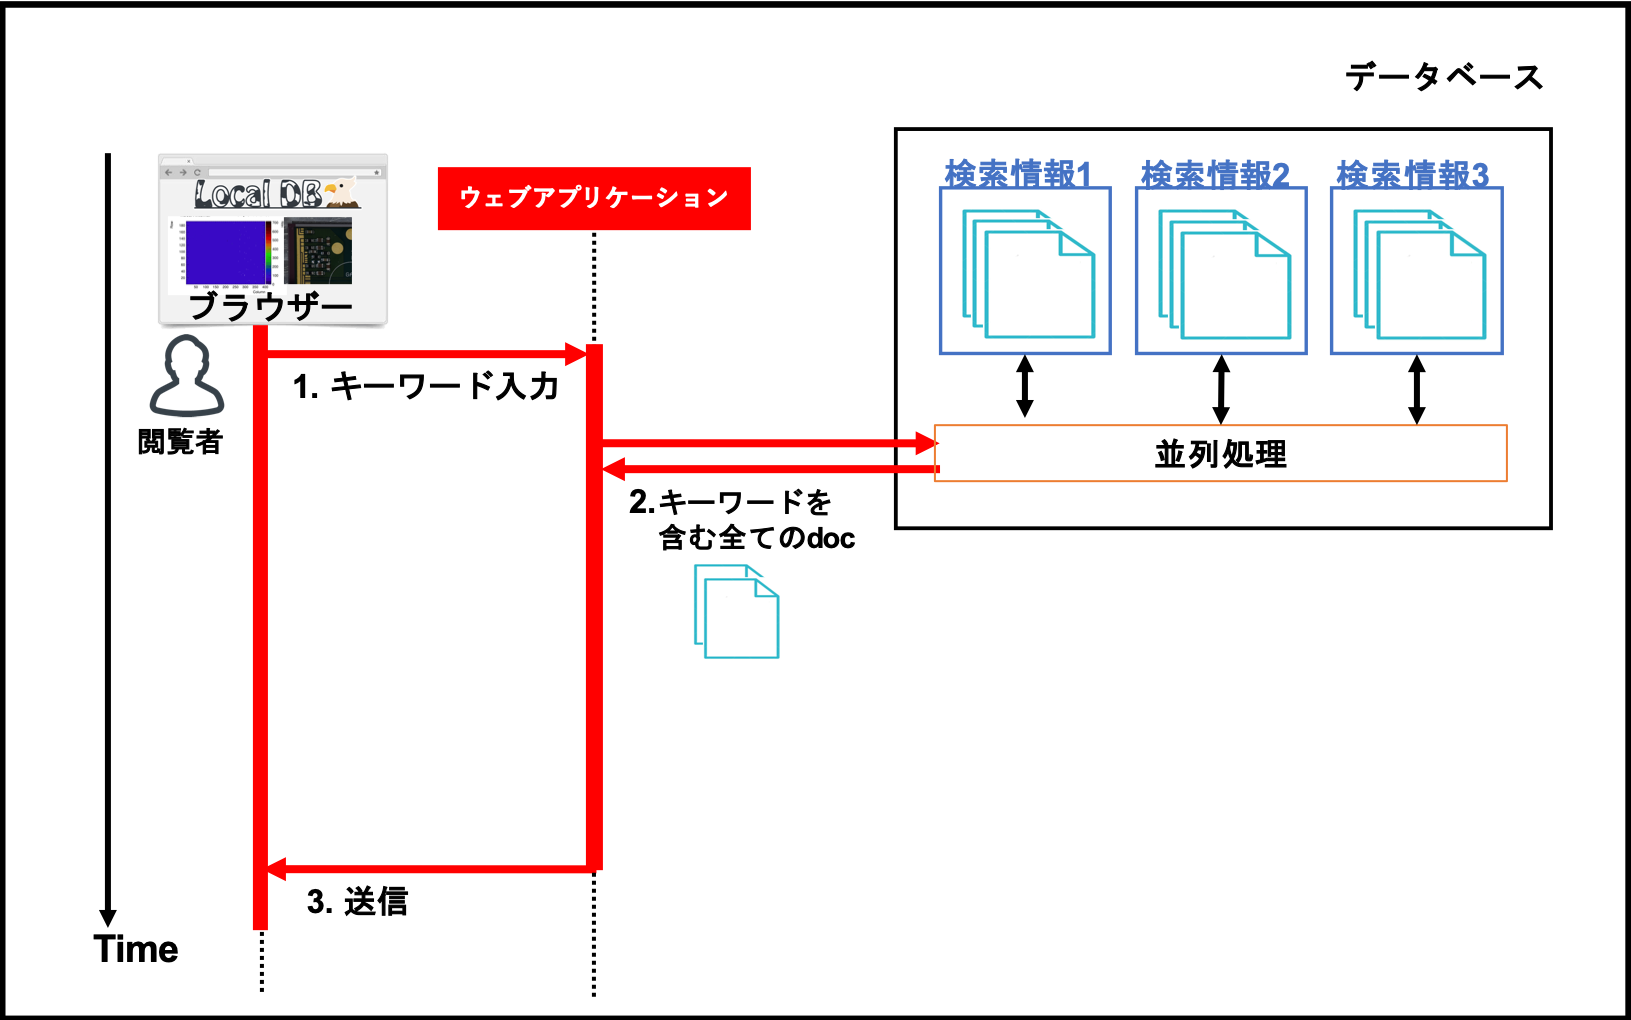
\includegraphics[width=12cm]{search_multi_thread}
  \caption[検索機能実装方法4:検索情報コレクションを分散、マルチスレッドを使用]{検索機能実装方法4:検索情報コレクションを分散、マルチスレッドを使用。方法3に加えて、検索情報コレクションを分散し、並列処理を行うことで、1つのコレクションあたりに含まれるドキュメント数を減らし、コレクション検索にかかる時間を削減できると考えられる。}
  \label{search_multi_thread}
  \end{center}
\end{figure}

方法3、4について、章\ref{sec:search_process_time_mes}と同じ内容の測定を行った。
方法2のものと合わせた結果を\ref{searching_time_2}に示す。
方法4について、分散するコレクション数は10個、スレッド数には2とした。
方法2に比べて、方法3、4共に処理時間が改善していることがわかる。

方法3、4を比べると傾きに差が見られる。そのため、方法4はドキュメント数が多くなった時に有効であると考えられる。
方法4に関しては今回はコレクション数を10、スレッド数を2としたが、それぞれ最適な数を検討することで更なる改善ができる可能性がある。

得られた方法3,4に関する関係を式\ref{function_summary_hash}、\ref{function_multi_thread}に示す。

\begin{figure}[bpt]
  \begin{center}
    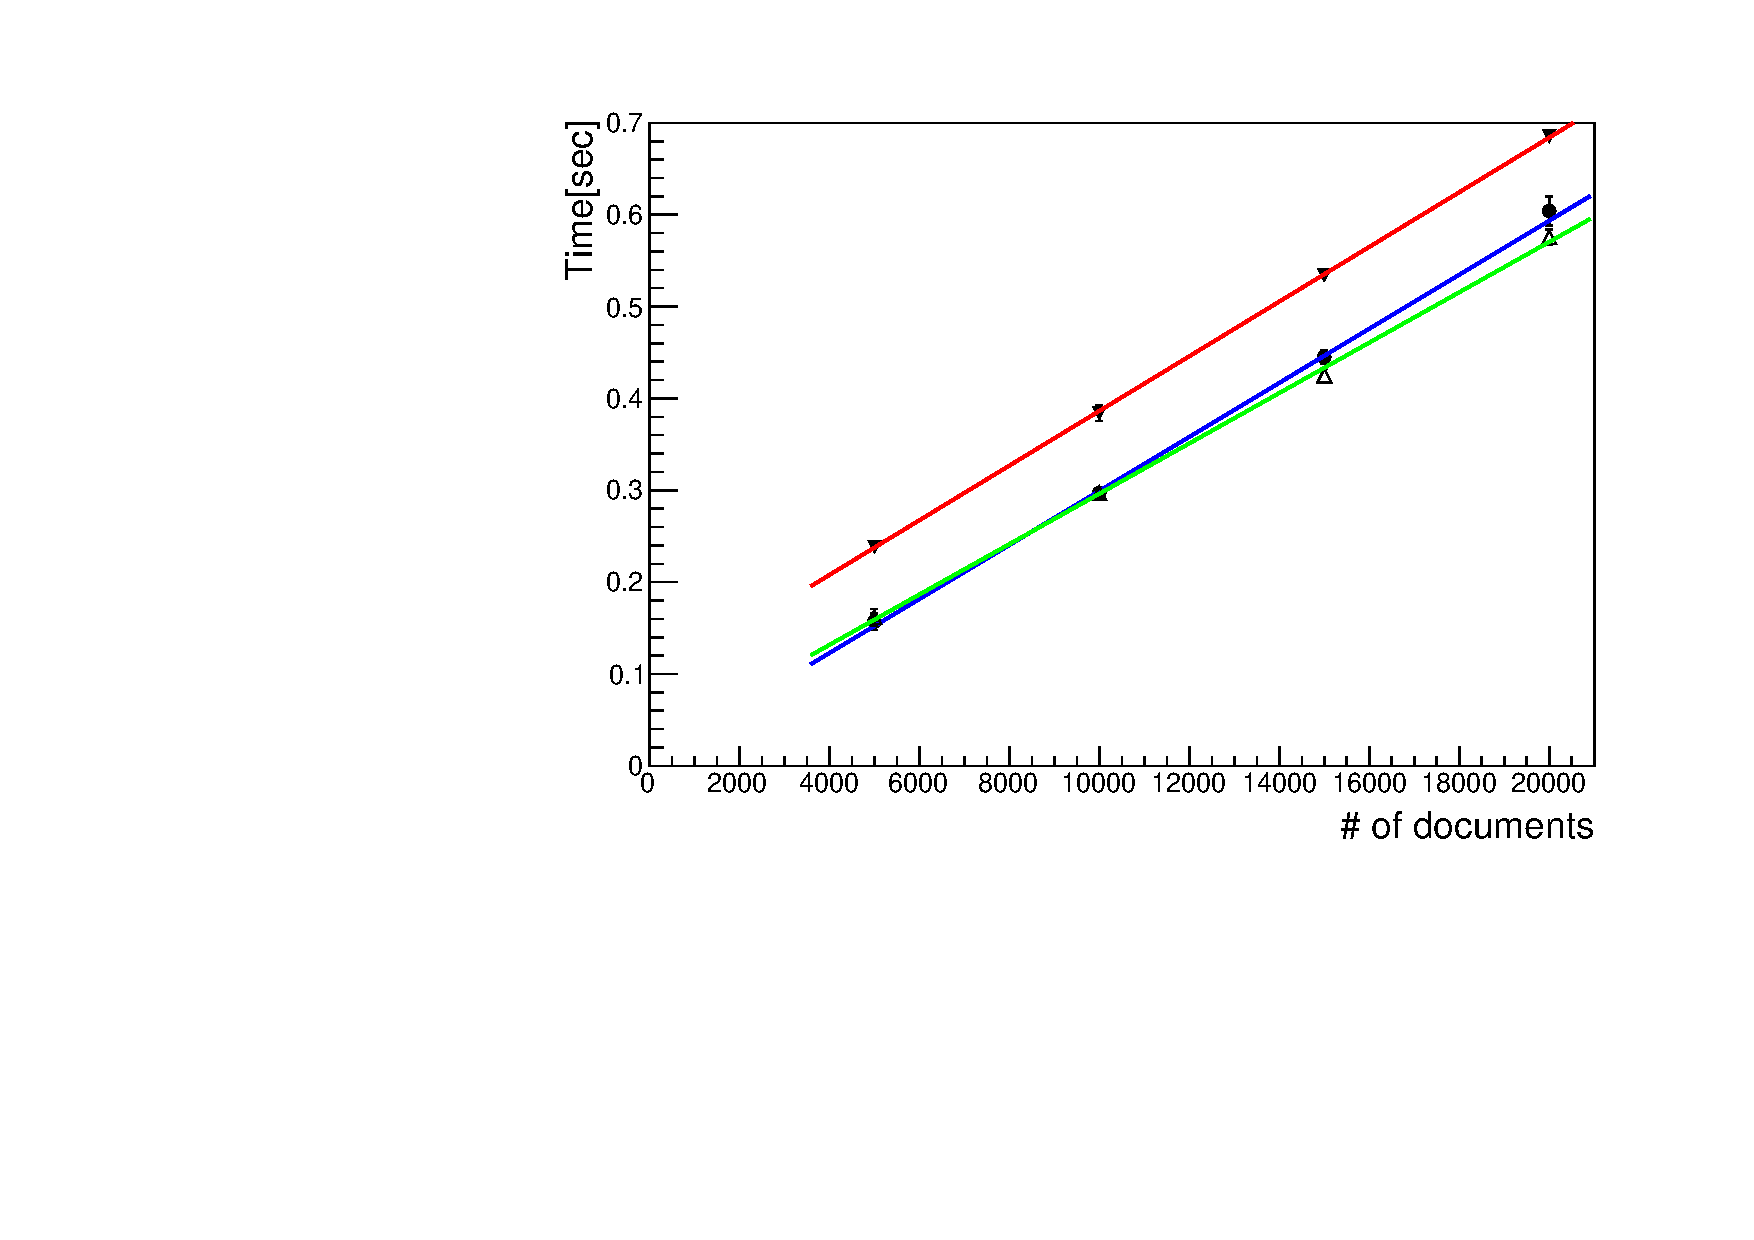
\includegraphics[width=8cm,angle=270]{searching_time_2.pdf}
  \caption[方法3、4に対する処理時間測定結果]{方法3、4に対する処理時間測定結果。横軸が試験結果のドキュメント数、縦軸が処理時間を表している。赤、青、緑がそれぞれ方法2、3、4を用いたものである。方法2に比べて3、4共に改善していることが分かる。方法3、4を比べると傾きが小さくなっていることが分かる。これよりドキュメント数が大きい場合に方法4は有効である。}
  \label{searching_time_2}
  \end{center}
\end{figure}

\bbb
y &=& ax + b \\
\label{function_summary_hash}
a &=& (2.9\pm0.1)\times10^{-5} \nonumber \\
b &=& (5.0\pm 1.1)\times10^{-3} \nonumber
\eee

\bbb
y &=& ax + b \\
\label{function_multi_thread}
a &=& (2.7\pm0.1)\times10^{-5} \nonumber \\
b &=& (2.2\pm 1.0)\times10^{-2} \nonumber
\eee

